\documentclass[a4paper, 11pt]{article}

\usepackage[a4paper,margin=1in]{geometry}
\usepackage[french]{babel}
\usepackage[utf8]{inputenc}
\usepackage[T1]{fontenc}
\usepackage{lmodern}
\usepackage{listings}
\usepackage{graphicx}
\usepackage{amsmath}
\usepackage{framed}
\usepackage{amsfonts}
\usepackage{caption}
\usepackage{subcaption}
\usepackage{listings}
\usepackage{color}
\usepackage[dvipsnames]{xcolor}
\usepackage{fancyhdr}
\usepackage{lastpage}


\graphicspath{{../imgs/}}


\definecolor{morange}{RGB}{237,106,90}
\definecolor{mgreen}{RGB}{63,127,95}
\definecolor{mpurple}{RGB}{127,0,85}

\lstset{
  basicstyle=\small\ttfamily, % Global Code Style
  captionpos=b, % Position of the Caption (t for top, b for bottom)
  extendedchars=true, % Allows 256 instead of 128 ASCII characters
  tabsize=2, % number of spaces indented when discovering a tab
  columns=fixed, % make all characters equal width
  keepspaces=true, % does not ignore spaces to fit width, convert tabs to spaces
  showstringspaces=false, % lets spaces in strings appear as real spaces
  breaklines=true, % wrap lines if they don't fit
  frame=trbl, % draw a frame at the top, right, left and bottom of the listing
  frameround=tttt, % make the frame round at all four corners
  framesep=4pt, % quarter circle size of the round corners
  numbers=left, % show line numbers at the left
  numberstyle=\tiny\ttfamily, % style of the line numbers
  commentstyle=\color{mgreen}, % style of comments
  keywordstyle=\color{mpurple}, % style of keywords
  stringstyle=\color{morange}, % style of strings
}

% TAILLE DES PAGES (A4 serré)

\setlength{\parindent}{0pt}
\setlength{\parskip}{1em}
%% \setlength{\textwidth}{17cm}
%% \setlength{\textheight}{24cm}
%% \setlength{\oddsidemargin}{-.7cm}
%% \setlength{\evensidemargin}{-.7cm}
%% \setlength{\topmargin}{-.5in}


\pagestyle{fancy}
\renewcommand{\headrulewidth}{0pt}
\renewcommand{\footrulewidth}{0.6pt}% default is 0pt
\lhead{}
\rhead{}
\lfoot{Page \thepage\ of \pageref{LastPage}}
\rfoot{Rémi Lespinet}
\cfoot{}
\cfoot{}



\newcounter{cquestion}[subsection]
\renewcommand{\thecquestion}{\alph{cquestion}}
\newenvironment{question}
{\par \vspace{0.5em} \noindent \stepcounter{cquestion} \hspace{-1em}
 \textbf{(\thecquestion)}}
{}

\newenvironment{note}
{\begin{framed} \textbf{Note : }}
{\end{framed}}


% Commandes de mise en page
\newcommand{\file}[1]{\emph{#1}}
\newcommand{\name}[1]{\emph{#1}}
\newcommand{\Fig}[1]{Fig \ref{#1} p. \pageref{#1}}
\newcommand{\Figure}[1]{Figure \ref{#1} p. \pageref{#1}}
\newcommand{\Tab}[1]{Tab \ref{#1} p. \pageref{#1}}
\newcommand{\Table}[1]{Table \ref{#1} p. \pageref{#1}}
\newcommand{\itemi}{\item[$\bullet$]}
% Commandes color
\newcommand{\colgood}[1]{\color{ForestGreen} #1}
\newcommand{\colbad}[1]{\color{BrickRed} #1}


% Commandes de maths
\newcommand{\function}[3]{#1 : #2 \to #3}
\newcommand{\intn}[2]{\left\{ #1 \dots #2 \right\}}
\newcommand{\intr}[2]{\left[ #1 ; #2 \right]}
\newcommand{\intro}[2]{\left] #1 ; #2 \right[}
\newcommand{\dotp}[2]{\langle #1, #2 \rangle}
\newcommand{\logn}[1]{\ln\left( #1\right)}
%% \newcommand{\det}[1]{\left| #1 \right|}
\newcommand{\pd}[2]{\frac{\partial #1}{\partial #2}}
\newcommand{\norm}[1]{\|#1\|}
\newcommand{\set}[2]{\left\{ #1 \hspace{.5em} ; \hspace{.5em}#2 \right\}}
\newcommand{\tr}[1]{Tr\left( #1 \right)}

\newcommand{\iid}{i.i.d }
\newcommand{\wrt}{w.r.t }

% Commandes informatique
\newcommand{\pfun}[1]{{\textbf{\texttt{#1}}}}

\newcommand{\ipart}[1]{\vspace{0.5em}\textbf{#1}\vspace{0.5em}}



\pagenumbering{arabic}

\title{\textsc{Graphical models - MVA 2017/2018 \\ \emph{Homework 1}} }
\author{Rémi Lespinet}
\date{}

\begin{document}

\maketitle
\thispagestyle{fancy}

\section{Learning in discrete graphical models}

Let $N \in \mathbb{N}$ and $\left(y^{(1)}, \dots, y^{(N)}\right)$ a sample
of observations. $\forall i \in \intn{1}{N}, y^{(i)} = (x^{(i)}, y^{(i)})$

\begin{equation*}
  \mathcal{L}(\theta, \pi) = p(y^{(1)}, \dots, y^{(N)} ; \theta, \pi)
\end{equation*}

By independance of the observations, we can write

\begin{align*}
  \mathcal{L}(\theta, \pi) & = \prod_{i = 1}^{N} p(y^{(i)}; \theta, \pi) \\
  %% & = \prod_{i = 1}^{N} p(x_i, z_i; \theta, \pi) \\
  & = \prod_{i = 1}^{N} p(x^{(i)} | z^{(i)}; \theta, \pi) p(z^{(i)}; \theta, \pi) \\
  & = \prod_{i = 1}^{N} \left( \prod_{m = 1}^M \prod_{k = 1}^K \theta_{m k}^{\hat{x}^{(i)}_{m k}} \right) \left( \prod_{m = 1}^M \pi_m^{\hat{z}^{(i)}_m} \right) \\
  & = \prod_{i = 1}^{N} \left( \prod_{m = 1}^M \left( \pi_m^{\hat{z}^{(i)}_m} \prod_{k = 1}^K \theta_{m k}^{\hat{x}^{(i)}_{m k}} \right) \right)
\end{align*}

where

\begin{equation*}
  \forall i \in \intn{1}{N}, \forall m \in \intn{1}{M}, \hat{z}^{(i)}_m = \left\{
  \begin{array}{l}
    1 \text{ if } z^{(i)} = m \\
    0 \text{ otherwise }
  \end{array}
  \right. \hspace{1em}\text{(One hot encoding)}
\end{equation*}

and

\begin{equation*}
  \forall i \in \intn{1}{N}, \forall m \in \intn{1}{M}, \forall k \in \intn{1}{K}, \hat{x}^{(i)}_{k m} = \left\{
  \begin{array}{l}
    1 \text{ if } z^{(i)} = m \land x^{(i)} = k \\
    0 \text{ otherwise }
  \end{array}
  \right.
\end{equation*}

If we write the log likelihood,

\begin{equation*}
  \ln{\mathcal{L}(\theta, \pi)} = \sum_{i = 1}^{N} \left( \sum_{m = 1}^M \left( \hat{z}^{(i)}_m \logn{\pi_m} + \sum_{k = 1}^K \hat{x}^{(i)}_{m k} \logn{\theta_{m k}} \right) \right)
\end{equation*}

This is a maximisation problem under the contraints
\begin{equation*}
  \left\{
  \begin{array}{l}
    \sum_{m = 1}^M \pi_m = 1 \\
    \forall m \in \intn{1}{M} \sum_{k = 1}^{K} \theta_{m k} = 1
  \end{array}
  \right.
\end{equation*}

We don't need to add the constraints $\pi_i > 0$ and $\theta_{m k} > 0$
because the expression of the log likelihood tends to $-\infty$
when one of the $\pi_i$ or $\theta_{m k}$ tends to $0$.

Writing the lagrangian, we get

\begin{equation*}
  L(\pi,\theta, \lambda, \mu) = - \ln{\mathcal{L}(\theta, \pi)} + \lambda \left( \sum_{m = 1}^M {\pi_m} - 1\right) + \sum_{m = 1}^M \mu_m \left( \sum_{k = 1}^K \theta_{m k}  - 1\right)
\end{equation*}

%% The lagrange dual function is
%% \begin{equation*}
%%   g(\lambda, \mu) = \inf_{\pi, \theta}{L(\pi,\theta, \lambda, \mu)}
%% \end{equation*}

Since the negative log likelihood is strictly convex with respect to
$\pi, \theta$, the lagrangian is also strictly convex with respect
to these variables and we know that there exist a minimum and that
it's unique.

Moreover there exists $(\pi_1, \dots \pi_M) \in \intr{0}{1}^M$ such that
\begin{equation*}
  \sum_{i = 1}^M \pi_i = 1
\end{equation*}

and $\theta \in \mathcal{M}_{M \times K}(\mathbb{R})$ such that

\begin{equation*}
  \forall m \in \intn{1}{M}, \sum_{k = 1}^K \theta_{m k} = 1
\end{equation*}

By Slater's constraint we have strong duality.

Let $j \in \intn{1}{M}$ and $l \in \intn{1}{K}$,

\begin{equation*}
  \pd{L}{\pi_j}(\pi,\theta, \lambda, \mu) = - \sum_{i = 1}^N \frac{z^{(i)}_j}{\pi_j} + \lambda = - \frac{\Phi_j}{\pi_j} + \lambda
\end{equation*}

where $\forall j \in \intn{1, M}, \Phi_j = \#\set{i}{z^{(i)} = j}$

\begin{equation*}
  \pd{L}{\theta_{l j}}(\pi,\theta, \lambda, \mu) = - \sum_{i = 1}^N \frac{x^{(i)}_{j l}}{\theta_{j l}} + \mu_j = \frac{\Psi_{j l}}{\theta_{j l}} + \mu_j
\end{equation*}

where $\forall j \in \intn{1}{M}, \forall l \in \intn{1}{K}, \Psi_{j l} = \#\set{i}{x^{(i)} = l \land z^{(i)} = j}$

At optimum, we have
\begin{equation*}
  \forall j \in \intn{1}{M}, \frac{\Phi_j}{\pi_j} = \lambda
\end{equation*}
and

\begin{equation*}
  \forall j \in \intn{1}{M}, \forall l \in \intn{1}{K}, \frac{\Psi_{j l}}{\theta_{j l}} = \mu_j
\end{equation*}

since
\begin{equation*}
  \forall j \in \intn{1}{M}, \sum_{j = 1}^M \pi_j = \sum_{j = 1}^M \frac{\Phi_j}{\lambda} = 1
\end{equation*}

We have $\lambda = N$. By applying the same reasonment,

\begin{equation*}
  \forall j \in \intn{1}{M}, \sum_{l = 1}^K \theta_{j l} = \sum_{l = 1}^K \frac{\Psi_{j l}}{\mu_j} = 1
\end{equation*}

which lead to $\mu_j = \#\set{i}{z^{(i)} = j}$



\begin{framed}
  \begin{align*}
    \forall m \in \intn{1}{M}, \hat{\pi}_m & = \frac{\#\set{i}{z^{(i)} = m}}{N} \\
    %% \end{equation*}
    %% \begin{equation*}
    \forall m \in \intn{1}{M}, \forall k \in \intn{1}{K}, \hat{\theta}_{m k} & = \frac{\#\set{i}{x^{(i)} = l \land z^{(i)} = j}}{\#\set{i}{z^{(i)} = j}}
  \end{align*}
\end{framed}

%% End exercice

\section{Linear classification}

\subsection{Generative model (LDA)}

\begin{question}
  The parameters for this model are $\pi$, $\mu_0$, $\mu_1$ and
  $\Sigma$.  Let $N$ be the number of observations in the sample,
  and let $\theta = \pi, \mu_0, \mu_1, \Sigma$, the parameters of the model.
  we can express the likelihood as follows
  \begin{equation*}
    \mathcal{L}(\theta) = p((x^{(1)}, y^{(1)}), ... (x^{(N)}, y^{(N)}) ; \theta)
  \end{equation*}
  We assume that the observations $(x^{(i)}, y^{(i)})$ are \iid.
  \begin{align*}
    \mathcal{L}(\theta) & = \prod_{i = 1}^N p(x^{(i)}, y^{(i)} ; \theta) \\
    & = \prod_{i = 1}^N p(x^{(i)} | y^{(i)} ; \theta) p(y^{(i)} ; \theta)
  \end{align*}

  We have
  \begin{equation*}
    p(y^{(i)} ; \pi) = \pi^{y^{(i)}} (1 - \pi)^{(1 - y^{(i)})}
  \end{equation*}
  and
  \begin{equation*}
    p(x^{(i)} | y^{(i)} ; \mu_i, \Sigma) = \dfrac{1}{\sqrt{(2\pi)^d \det{\Sigma}}} \exp{\left( -\dfrac{1}{2} (x^{(i)} - \mu_{y^{(i)}})^T \Sigma^{-1} (x^{(i)} - \mu_{y^{(i)}}) \right)}
  \end{equation*}

  The log likelihood is then expressed as

  \begin{align*}
    \ln{\mathcal{L}(\theta)} & = \sum_{i = 1}^N y^{(i)} \ln{(\pi)} + (1 - y^{(i)})\ln{(1 - \pi)} - \dfrac{1}{2}\ln{((2\pi)^d \det{\Sigma})} - \dfrac{1}{2}(x^{(i)} - \mu_{y^{(i)}})^T \Sigma^{-1} (x^{(i)} - \mu_{y^{(i)}}) \\
    & = \sum_{i = 1}^N y^{(i)} \ln{(\pi)} + (1 - y^{(i)})\ln{(1 - \pi)} - \dfrac{d}{2}\ln{(2\pi)} - \dfrac{1}{2}\ln{(\det{\Sigma})} - \dfrac{1}{2}(x^{(i)} - \mu_{y^{(i)}})^T \Sigma^{-1} (x^{(i)} - \mu_{y^{(i)}}) \\
  \end{align*}

  \ipart{Maximum likelihood estimator for $\pi$}

  The log likelihood is strictly concave \wrt $\pi$, so finding the
  maximum likelihood estimator for $\pi$ is of finding $\pi$ which
  satisfies partial derivate \wrt $\pi$.

  \begin{align*}
    \pd{}{\pi}\ln{\mathcal{L}}(\theta) & = \sum_{i = 1}^N \dfrac{y^{(i)}}{\pi} - \dfrac{(1 - y^{(i)})}{(1 - \pi)} \\
    & = \dfrac{N_1}{\pi} - \dfrac{N_0}{(1 - \pi)}
  \end{align*}


  Where $N_1 = \sum_{i = 1}^N y^{(i)}$ and $N_0 = \sum_{i = 1}^N (1 - y^{(i)})$ (we have $N_0 + N_1 = N$)

  \begin{align*}
    \pd{}{\pi}\ln{\mathcal{L}}(\theta) = 0 & \Leftrightarrow \dfrac{N_1}{\pi} = \dfrac{N_0}{(1 - \pi)} \\
    & \Leftrightarrow \pi N_0 = (1 - \pi) N_1 \\
    & \Leftrightarrow \pi = \frac{N_1}{N}
  \end{align*}

  \ipart{Maximum likelihood estimator for $\mu_j$}

  Let $j \in \left\{0, 1\right\}$. Because $\Sigma$ is supposed
  definite, $\Sigma^{-1}$ is also definite (if $\Sigma$ is only
  supposed semi-definite, it may not be invertible).
  \begin{align*}
    \nabla_{\mu_j}{\ln{\mathcal{L}}}(\theta) & = - \sum_{i = 1}^N \delta_{(y^{(i)},j)} 2 \Sigma^{-1} (x^{(i)} - \mu_j) \\
    & = 2 \Sigma^{-1} (S_j - N_j \mu_j)
  \end{align*}

  Where
  \begin{equation*}
    \forall i, j \in \left\{0, 1\right\} \delta_{(i,j)} = \left\{
    \begin{array}{l}
      1 \text{ if } i = j \\
      0 \text{ otherwise }
    \end{array}
    \right.
  \end{equation*}

  $S_j$ is the sum of the observations $x^{(i)}$ such that $y^{(i)}$
  is is $j$, or more formally
  \begin{equation*}
    S_j = \sum_{i = 1}^N \delta_{(y^{(i)},j)} x^{(i)}
  \end{equation*}
  And $N_j$ is the number of $i$ such that $y^{(i)}$ is $j$ (as in the previous section)
  \begin{equation*}
    N_j = \sum_{i = 1}^N \delta_{(y^{(i)},j)}
  \end{equation*}

  We then have

  \begin{align*}
    \nabla_{\mu_j}\ln{\mathcal{L}}(\theta) = 0 & \Leftrightarrow 2 \Sigma^{-1} (S_j - N_j\mu_j) = 0
  \end{align*}

  Since $\Sigma^{-1}$ is definite,

  \begin{align*}
    \nabla_{\mu_j}\ln{\mathcal{L}}(\theta) = 0 & \Leftrightarrow \mu_j = \frac{S_j}{N_j} = \bar{x}_j
  \end{align*}

  With $\bar{x}_j$ being the mean of the $x^{(i)}$ such that $y^{(i)} = j$

  \ipart{Maximum likelihood estimator for $\Sigma$}

  \begin{equation*}
    \nabla_{\Sigma}\ln{\mathcal{L}}(\theta) = \pd{}{\Sigma}\left( - \dfrac{N}{2}\ln{(\det{\Sigma})} - \dfrac{1}{2} \sum_{i = 1}^N (x^{(i)} - \mu_{y^{(i)}})^T \Sigma^{-1} (x^{(i)} - \mu_{y^{(i)}}) \right)
  \end{equation*}


  Let $\Omega = \Sigma^{-1}$ and let $g$ the function such that

  \begin{equation*}
    g_{\pi, \mu_0, \mu_1}(\Omega) = L(\pi, \mu_0, \mu_1, \Omega^{-1})
  \end{equation*}

  Which we can rewrite

  \begin{equation*}
    \begin{split}
      \nabla_{\Sigma}\ln{\mathcal{L}}(\theta) = \nabla_{\Sigma} \Biggl(
      & - \dfrac{N}{2}\ln{(\det{\Sigma})} \\
      & - \dfrac{1}{2} \sum_{i = 1}^N y^{(i)} (x^{(i)} - \mu_1)^T \Sigma^{-1} (x^{(i)} - \mu_1) \\
      & - \dfrac{1}{2} \sum_{i = 1}^N (1 - y^{(i)}) (x^{(i)} - \mu_0)^T \Sigma^{-1} (x^{(i)} - \mu_0)
      \Biggr)
    \end{split}
  \end{equation*}

  Since

  \begin{align*}
    \sum_{i = 1}^N (x^{(i)} - \mu_j)^T \Sigma^{-1} (x^{(i)} - \mu_j) & = \sum_{i = 1}^N \tr{(x^{(i)} - \mu_j)^T \Sigma^{-1} (x^{(i)} - \mu_j)} \\
    & = \sum_{i = 1}^N \tr{\Sigma^{-1} (x^{(i)} - \mu_j) (x^{(i)} - \mu_j)^T}
  \end{align*}

  We know that
  \begin{equation*}
    \nabla_{\Sigma^{-1}}\ln{(\det{\Sigma^{-1}})} = \Sigma
  \end{equation*}

  If we take the gradient with respect to $\Sigma^{-1}$, we obtain
  \begin{equation*}
    \nabla_{\Sigma^{-1}}\ln{\mathcal{L}}(\theta) = \dfrac{N}{2}\Sigma - \dfrac{1}{2} \sum_{i = 1}^N y_i (x^{(i)} - \mu_1)^T (x^{(i)} - \mu_1) - \dfrac{1}{2} \sum_{i = 1}^N (1 - y_i) (x^{(i)} - \mu_0)^T (x^{(i)} - \mu_0)
  \end{equation*}

  which is $0$ when
  \begin{align*}
    \Sigma & = \dfrac{1}{N} \left( \sum_{i = 1}^N y_i (x^{(i)} - \mu_1)^T (x^{(i)} - \mu_1) + \sum_{i = 1}^N (1 - y_i) (x^{(i)} - \mu_0)^T (x^{(i)} - \mu_0) \right) \\
    & = \dfrac{1}{N} \sum_{i = 1}^N (x^{(i)} - \mu_{y_i})^T (x^{(i)} - \mu_{y_i})
  \end{align*}

  \textbf{Conclusion}

  \begin{framed}
    \begin{align*}
      \hat{\pi}_{MLE} & = \dfrac{S_j}{N_j} \\
      \hat{\mu_j}_{MLE} & = \dfrac{S_j}{N_j} \\
      \hat{\Sigma}_{MLE} & = \dfrac{1}{N} \sum_{i = 1}^N (x^{(i)} - \mu_{y_i})^T (x^{(i)} - \mu_{y_i})
    \end{align*}
  \end{framed}



\end{question}

\begin{question}
  We suppose $0 < \pi < 1$. From bayes rule, we have
  \begin{align*}
    p(y = 1 | x) & = \dfrac{p(x | y = 1) p(y = 1)}{p(x | y = 1) p(y = 1) + p(x | y = 0) p(y = 0)} \\
    & = \dfrac{1}{1 + \dfrac{p(x | y = 0) p(y = 0)}{p(x | y = 1) p(y = 1)}}
  \end{align*}

  Since we have
  \begin{equation*}
    p(x | y = i) = \frac{1}{\sqrt{(2\pi)^d \det{\Sigma}}} \exp{\left(-\dfrac{1}{2}(x - \mu_i)^T \Sigma^{-1} (x - \mu_i)\right)}
  \end{equation*}

  We can write

  \begin{align*}
    \dfrac{p(x | y = 0) p(y = 0)}{p(x | y = 1) p(y = 1)}
    & = \dfrac{\pi - 1}{\pi} \exp{\left(-\frac{1}{2} \left( (x - \mu_0)^T \Sigma^{-1} (x - \mu_0) - (x - \mu_1)^T \Sigma^{-1} (x - \mu_1) \right)\right)} \\
    & = \dfrac{\pi - 1}{\pi} \exp{\left(-\frac{1}{2} \left( 2 x^T \Sigma^{-1} (\mu_0 - \mu_1) + \mu_0^T \Sigma^{-1} \mu_0 - \mu_1^T \Sigma^{-1} \mu_1 \right)\right)} \\
    & = \exp{\left(-\frac{1}{2} \left( 2 x^T \Sigma^{-1} (\mu_0 - \mu_1) + \mu_0^T \Sigma^{-1} \mu_0 - \mu_1^T \Sigma^{-1} \mu_1  + 2 \ln{(\pi)}- 2 \ln{(\pi - 1)}\right)\right)} \\
    & = \exp{\left( x^T \omega + \beta \right)}
  \end{align*}

  With $\omega = \Sigma^{-1} (\mu_1 - \mu_0)$ and
  $\beta = -\dfrac{1}{2} \left( \mu_0^T \Sigma^{-1} \mu_0 + \mu_1^T \Sigma^{-1} \mu_1 \right) + \ln{(\pi - 1)} - \ln{(\pi)}$

\end{question}

\begin{question}
  I've implemented a class LDA in the file \file{classify.py}.
  The function \pfun{train} is used to learn the parameters of
  the model and the function \pfun{probability} is used to predict
  the probability given samples

  %% TODO change probability function

  %% \begin{lstlisting}[language=Python]
  %%   class LDA(ClassificationModel):

  %%   def train(self, X, Y):
  %%   X0 = X[Y == 0]
  %%   X1 = X[Y == 1]
  %%   self.pi = np.mean(Y)
  %%   self.mu0 = np.mean(X0, axis=0)
  %%   self.mu1 = np.mean(X1, axis=0)
  %%   self.sigma = np.cov(np.r_[X0 - self.mu0, X1 - self.mu1].T)
  %%   self.sigmainv = np.linalg.inv(self.sigma)

  %%   def probability(self, X):
  %%   X0 = (X - self.mu0)
  %%   X1 = (X - self.mu1)
  %%   P0 = (1 - self.pi) * np.exp(-0.5 * X0.dot(self.sigmainv).dot(X0))
  %%   P1 = self.pi * np.exp(-0.5 * X1.dot(self.sigmainv).dot(X1))
  %%   return 1 / (1 + P0/P1)

  %% \end{lstlisting}


  From the previous question, we can obtain the expression of the
  line defined by $p(y = 1 | \theta)$
  \begin{align*}
    p(y = 1 | x) = \dfrac{1}{2} & \Leftrightarrow \dfrac{1}{1 + \exp{(\omega^T x + \beta)}} = \dfrac{1}{2} \\
    & \Leftrightarrow \exp{(\omega^T x + \beta)} = 1 \\
    & \Leftrightarrow \omega^T x + \beta = 0
  \end{align*}

  \begin{note}
    I could have implemented the drawing of the line using this
    equation (In fact, I dit it at the beginning and it worked
    well), but I later faced the problem of drawing quadratic
    curve for the QDA, and I found the magic function \pfun{contour}
    which is very easy to use, and provides fancy result so I used it
    to draw every curves in order to have homogeneous figures. (The code
    is still available as a comment in the file \file{classify.py}
  \end{note}

  The sample data and decision boundary of this classifier are
  represented on \Figure{fig:LDA}.  We define the
  \emph{training error} (resp. the \emph{test error}) as the ratio
  of observations in the training data (resp. in the test data) that
  are wrongly predicted by our predictor.

  The parameters learnt for this methods are presented in the
  \Table{tab:ParamLDA}.

  \begin{table}[h!]
    \centering
  \begin{tabular}{| l | l | l | l | c |}
    \hline
    sample file & $\pi$ & $\mu_0$ & $\mu_1$ & $\Sigma$ \\
    \hline
    \file{classificationA} &
    0.33 & (2.90, -0.89) & (-2.69, 0.87) &
    \( \left( \begin{array}{cc}
      2.46 & -1.14 \\
      -1.14 & 0.62
    \end{array} \right) \) \\

    \file{classificationB} &
    0.5 & (3.34, -0.84) & (-3.21, 1.08) &
    \( \left( \begin{array}{cc}
      3.36 & -0.14 \\
      -0.14 & 1.74
    \end{array} \right)  \) \\

    \file{classificationC} &
    0.625 & (2.79, -0.84) & (-2.94, -0.96) &
    \( \left( \begin{array}{cc}
      2.89 & -0.64 \\
      -0.64 & 5.21
    \end{array} \right)  \) \\
    \hline
  \end{tabular}
  \captionof{table}{Parameters learnt for the LDA method for the different training sample} \label{tab:ParamLDA}
\end{table}


  %% \begin{center}
  %%   \begin{tabular}{| l | l | l |}
  %%     \hline
  %%     sample file & train error & test error \\
  %%     \hline
  %%     \file{classificationA} & $1.33\%$ & $2.00\%$ \\
  %%     \file{classificationB} & $3.00\%$ & $4.15\%$ \\
  %%     \file{classificationC} & $5.50\%$ & $4.23\%$ \\
  %%     \hline
  %%   \end{tabular}
  %% \end{center}

  \begin{figure}[p]
    \centering
    \begin{subfigure}[t]{0.40\textwidth}
      \centering
      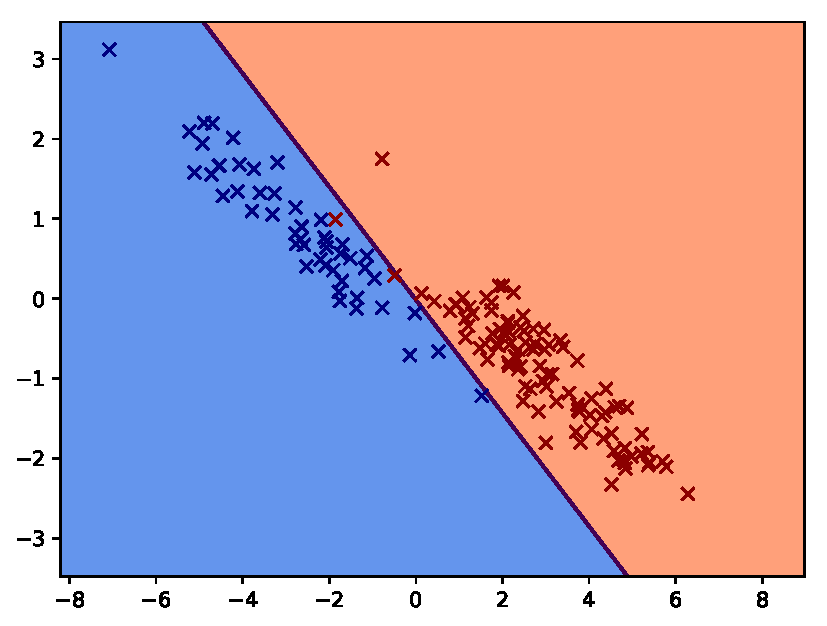
\includegraphics[width=\textwidth]{LDA_classificationA_train.pdf}
      \caption{Training observations A ($150$ points)}\label{fig:LDA-A-train}
    \end{subfigure}
    \quad
    \begin{subfigure}[t]{0.40\textwidth}
      \centering
      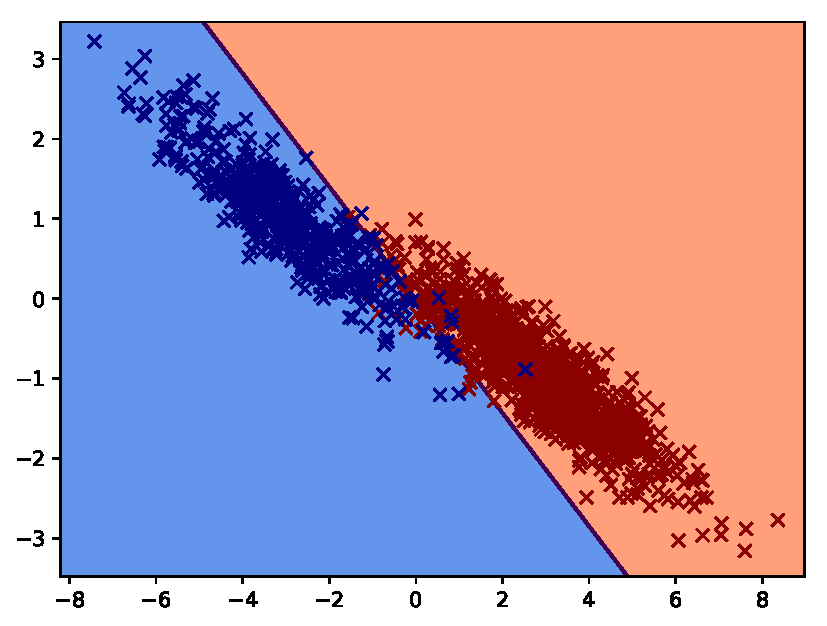
\includegraphics[width=\textwidth]{LDA_classificationA_test.pdf}
      \caption{Test observations A ($1500$ points)}\label{fig:LDA-A-test}
    \end{subfigure}
    \vskip\baselineskip
    \begin{subfigure}[t]{0.40\textwidth}
      \centering
      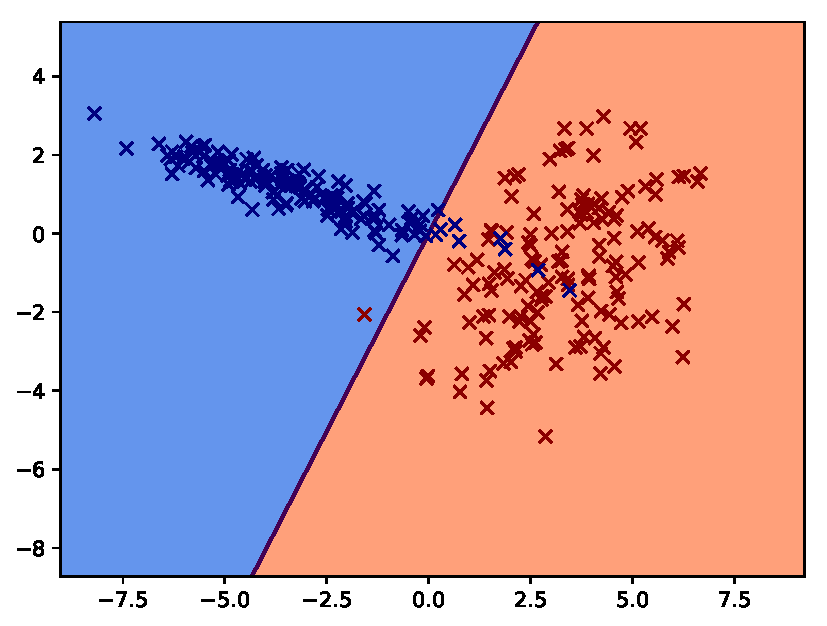
\includegraphics[width=\textwidth]{LDA_classificationB_train.pdf}
      \caption{Training observations B ($150$ points)}\label{fig:LDA-B-train}
    \end{subfigure}
    \quad
    \begin{subfigure}[t]{0.40\textwidth}
      \centering
      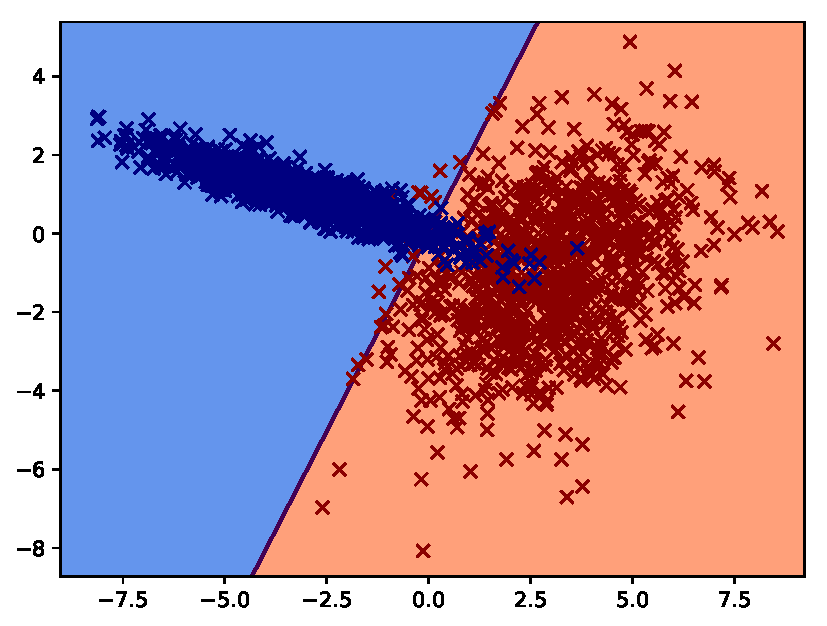
\includegraphics[width=\textwidth]{LDA_classificationB_test.pdf}
      \caption{Test observations B ($1500$ points)}\label{fig:LDA-B-test}
    \end{subfigure}
    \vskip\baselineskip
    \begin{subfigure}[t]{0.40\textwidth}
      \centering
      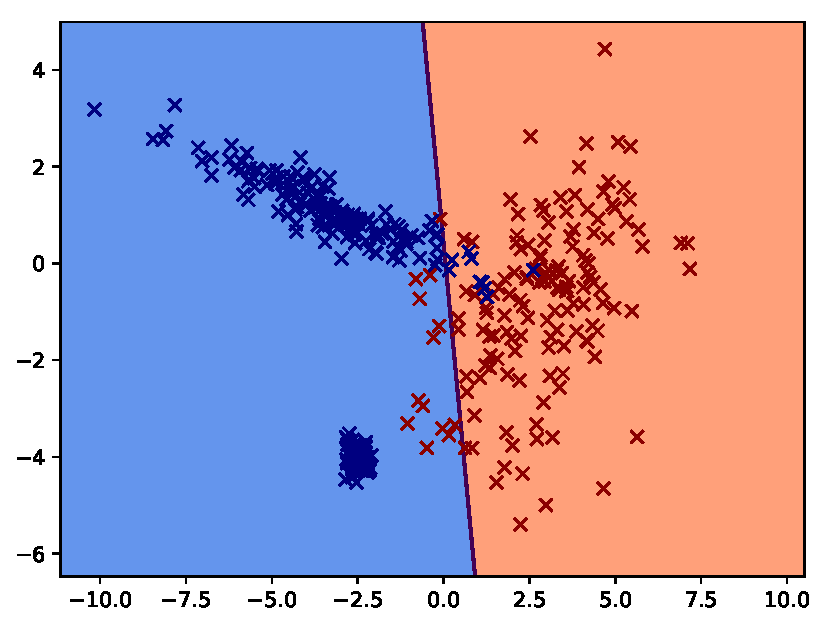
\includegraphics[width=\textwidth]{LDA_classificationC_train.pdf}
      \caption{Training observations C ($150$ points)}\label{fig:LDA-C-train}
    \end{subfigure}
    \quad
    \begin{subfigure}[t]{0.40\textwidth}
      \centering
      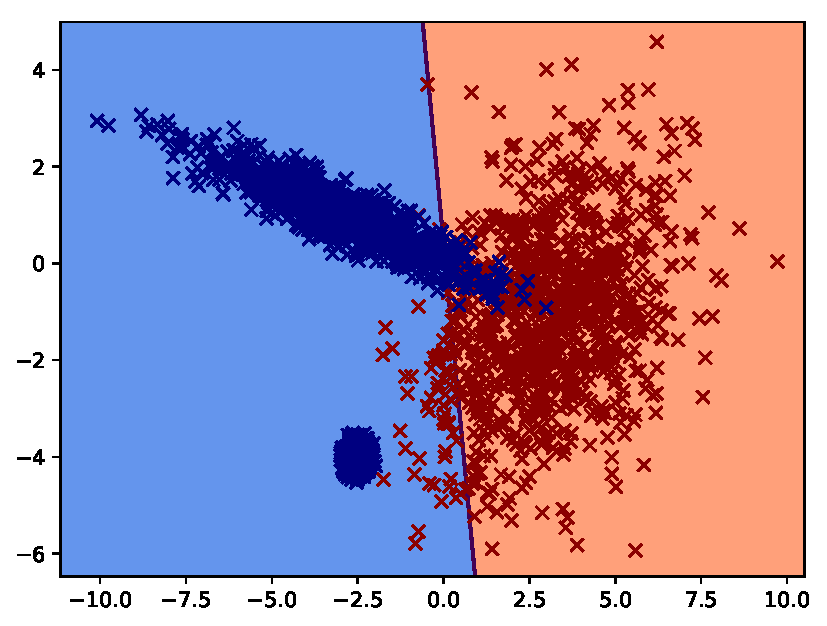
\includegraphics[width=\textwidth]{LDA_classificationC_test.pdf}
      \caption{Test observations C ($1500$ points)}\label{fig:LDA-C-test}
    \end{subfigure}
    \caption{Sample data and decision boundary representation for the LDA classifier on the three files}\label{fig:LDA}
  \end{figure}


\end{question}

\subsection{Logistic regression}
I have implemented the logistic regression using the
Newton-Raphson method (IRLS) as suggested.

If we note

\begin{equation*}
  \forall i \in \intn{1}{N}, n_i = \sigma(w^T x_i)
\end{equation*}

The update equation is

\begin{equation*}
  w_{t + 1} = w_t + Hl(w_t)^{-1} \nabla l(w)
\end{equation*}

with

\begin{align*}
  & l(w) = \sum_{i = 1}^N \left(y_i \ln{(\sigma(w^T x))} + (1 - y_i) \ln{(1 - \sigma{(w^T x)})} \right) \\
  & Hl(w) = -X^T diag(n \odot (1_{\mathbb{R}^N} - n)) X \\
  & \nabla l(w) = X^T (y - n)
\end{align*}

\begin{note}
  I've taken these equations from the lecture notes, to apply them, we need
  to add a column vectors of $1$ to X, for the affine part

  $\odot$ is the hadamar product of two matrices.
\end{note}

For the implementation, I used $10$ iterations, and an initial
vector of zeros. The parameters learnt are presented in the \Table{tab:ParamLogReg}

\begin{table}[h!]
  \centering
  \begin{tabular}{| l | l | l |}
    \hline
    sample file & $w$ \\
    \hline
    \file{classificationA} & $(42.63, 73.03, 7.80)$ \\
    \file{classificationB} & $(1.71, -1.02, -1.35)$ \\
    \file{classificationC} & $(2.20, -0.71, -0.96)$ \\
    \hline
  \end{tabular}
  \captionof{table}{Parameters learnt for the different training sample (no regularization)} \label{tab:ParamLogReg}
\end{table}

We observe that for the \file{classificationA}, $\norm{w}$ tends
to $\infty$. This is due to the fact that the data are separable,
We have

\begin{equation*}
  p(y = 1 | x) = p \Leftrightarrow w^T x = \ln{\left( \dfrac{1 - p}{p} \right)}
\end{equation*}

So the line $p(y = 1 | x) = 0.5$ is the same when we multiply $w$
by a constant $\alpha \in \mathbb{R}$, but for a fixed
$p \in \intr{0}{1}$, by multiplying $w$ by $\alpha$, we obtain

\begin{align*}
  \alpha  w^T x & = \alpha \ln{\left( \dfrac{1 - p}{p} \right)} \\
  & = \ln{\left(\left( \dfrac{1}{p} - 1\right)^\alpha\right)}
\end{align*}

If we consider $q$ such that
\begin{align*}
  \dfrac{1}{q} - 1 = \left( \dfrac{1}{p} - 1\right)^\alpha \Leftrightarrow q = \dfrac{p^\alpha}{p^\alpha + (1 - p)^\alpha}
\end{align*}

Which means that by multiplying $w$ by $\alpha$, the line
$p(y = 1 | x) = p$ becomes the line
\begin{equation*}
  p(y = 1 | x) = \dfrac{p^\alpha}{p^\alpha + (1 - p)^\alpha}
\end{equation*}

If we plot the function $f_\alpha : p \rightarrow \dfrac{p^\alpha}{p^\alpha + (1 - p)^\alpha}$,
(see \Fig{fig:scaleW}) we see that for $\alpha > 1$


\begin{figure}[h]
\centering
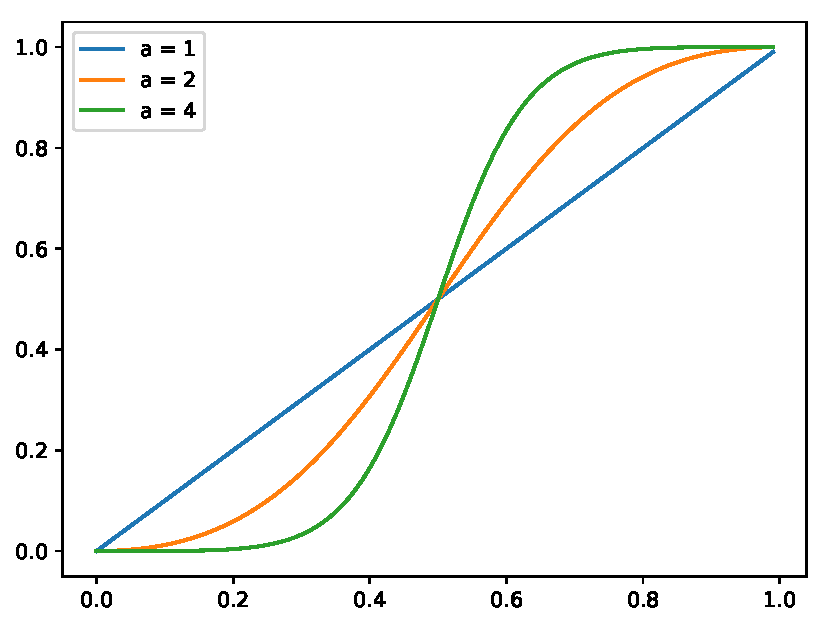
\includegraphics[width=0.5\textwidth]{scaleW.pdf}
\caption{Representation of $f_\alpha$ for different $\alpha$}
\label{fig:scaleW}
\end{figure}



\begin{equation*}
  \begin{array}{l}
    f(p) > p \text{ if } p > 0.5 \\
    f(p) < p \text{ if } p < 0.5 \\
  \end{array}
\end{equation*}

and also,

\begin{equation*}
  \lim_{\alpha \rightarrow \infty}f_\alpha(p) =
  \left\{
  \begin{array}{lll}
    0 &\text{if } &p < 0.5 \\
    0.5 &\text{if } &p = 0.5 \\
    1 &\text{if } &p > 0.5 \\
  \end{array}
  \right.
\end{equation*}

When the data is separable, the best solution is obviously to take
$w$ such that the hyperplane $w^T x = 0$ separates the data, and
make $\norm{w}$ tend to infinity such that all the observations
$x$ are such that $p(y = 1 | x) = 0$ or $p(y = 1 | x) = 1$
depending on whether they are located on one side of the half
space (supported by the hyperplan) or the other. On the
\Figure{fig:W} I have plotted the value of $p(y = 1 | x)$
on the entire plane, and we see the effect of multiplying $w$ by $a > 1$
graphicaly.

We can avoid this effect by introducing a regularization term, e.g
minimizing

\begin{equation*}
  \tilde{l}(w) = \sum_{i = 1}^N \left(y_i \ln{(\sigma(w^T x))} + (1 - y_i) \ln{(1 - \sigma{(w^T x)})} \right) + \dfrac{\lambda}{2} \norm{w}^2
\end{equation*}

\begin{note}
  I've implemented this regularization method with a parameter
  $\lambda = 0.001$ in the file \file{classify.py}. This gives
  the same values for the parameters and misclassification error
\end{note}


\begin{figure}[!ht]
  \centering
  \begin{subfigure}{.45\textwidth}
    \centering
    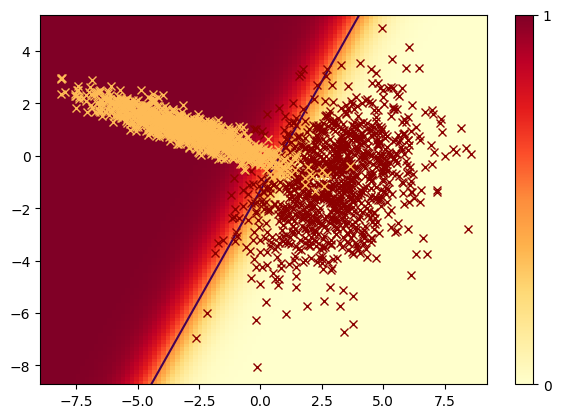
\includegraphics[width=1\linewidth]{W_times_1.png}
    \caption{$a = 1$ (w unchanged)}
    \label{fig:W1}
  \end{subfigure}%
  \begin{subfigure}{.45\textwidth}
    \centering
    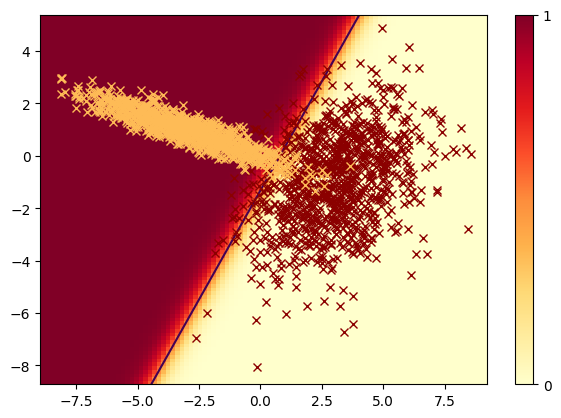
\includegraphics[width=1\linewidth]{W_times_2.png}
    \caption{$a = 2$}
    \label{fig:W2}
  \end{subfigure}%
  \vskip\baselineskip
  \begin{subfigure}{.45\textwidth}
    \centering
    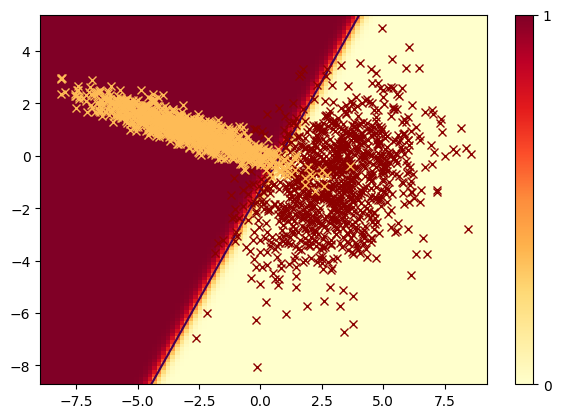
\includegraphics[width=1\linewidth]{W_times_4.png}
    \caption{$a = 4$}
    \label{fig:W4}
  \end{subfigure}%
  \caption{Representation of the variation of the probability $p(y = 1 | x)$ over the entire plane for the logistic regression when multiplying $w$ by a constant term $a$ (file \file{classificationB})}
  \label{fig:W}
\end{figure}

%% \begin{minipage}{\linewidth}
%%   \begin{lstlisting}[language=Python]
%%     class LogisticRegression(ClassificationModel):

%%     def train(self, X, Y):
%%     N = np.shape(X)[0]
%%     X = np.c_[X, np.ones(N)]
%%     self.W = self.W0.copy()
%%     for i in range(self.it):
%%     Xt = np.transpose(X)
%%     n = 1 / (1 + np.exp(np.dot(X, self.W)))
%%     D = np.diag(n * (1 - n))
%%     H = -np.dot(np.dot(Xt, D), X)
%%     G = np.dot(Xt, Y - n)
%%     self.W += np.dot(np.linalg.inv(H), G)


%%     def probability(self, X):
%%     X = np.hstack((X, 1))
%%     return 1 / (1 + np.exp(self.W.dot(X)))
%%   \end{lstlisting}
%% \end{minipage}


\begin{figure}[p]
  \centering
  \begin{subfigure}[t]{0.40\textwidth}
    \centering
    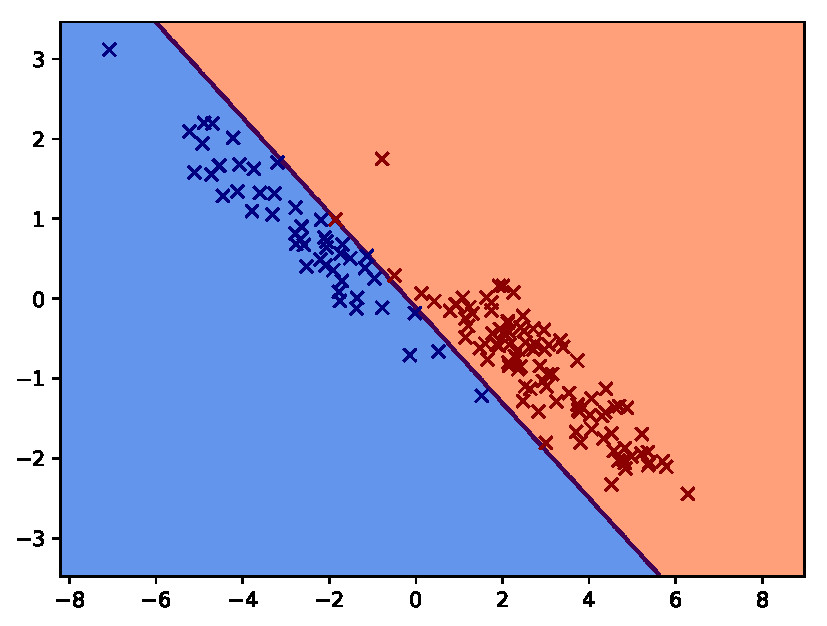
\includegraphics[width=\textwidth]{LogReg_classificationA_train.pdf}
    \caption{Training observations A ($150$ points)}\label{fig:LogReg-A-train}
  \end{subfigure}
  \quad
  \begin{subfigure}[t]{0.40\textwidth}
    \centering
    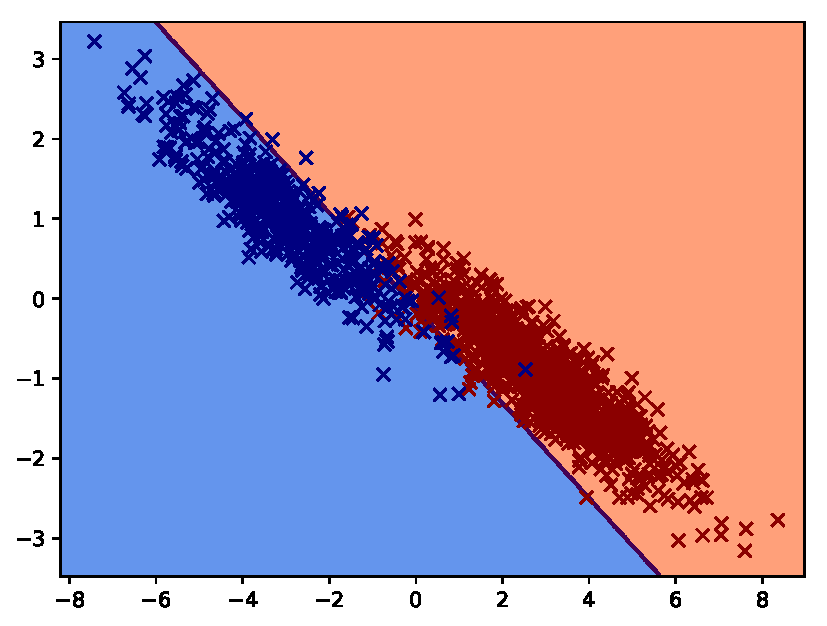
\includegraphics[width=\textwidth]{LogReg_classificationA_test.pdf}
    \caption{Test observations A ($1500$ points)}\label{fig:LogReg-A-test}
  \end{subfigure}
  \vskip\baselineskip
  \begin{subfigure}[t]{0.40\textwidth}
    \centering
    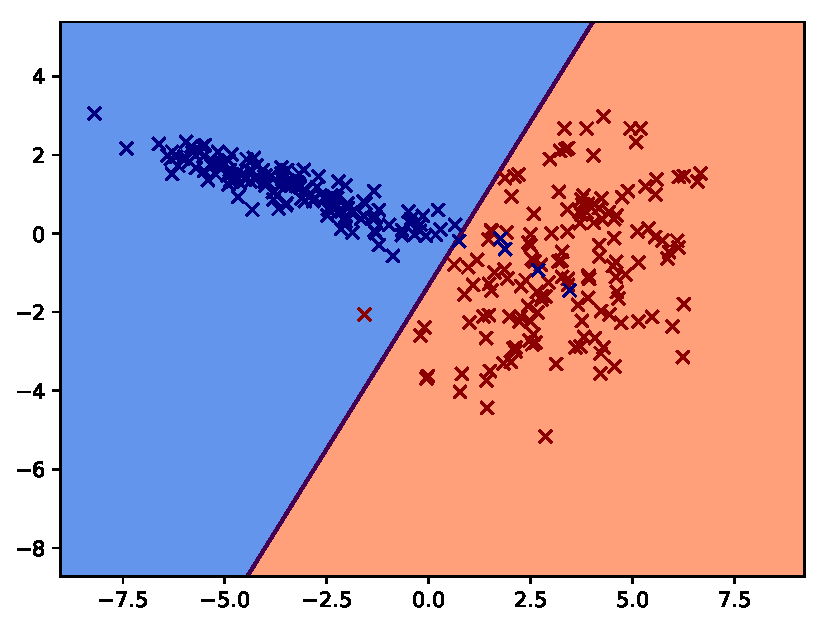
\includegraphics[width=\textwidth]{LogReg_classificationB_train.pdf}
    \caption{Training observations B ($150$ points)}\label{fig:LogReg-B-train}
  \end{subfigure}
  \quad
  \begin{subfigure}[t]{0.40\textwidth}
    \centering
    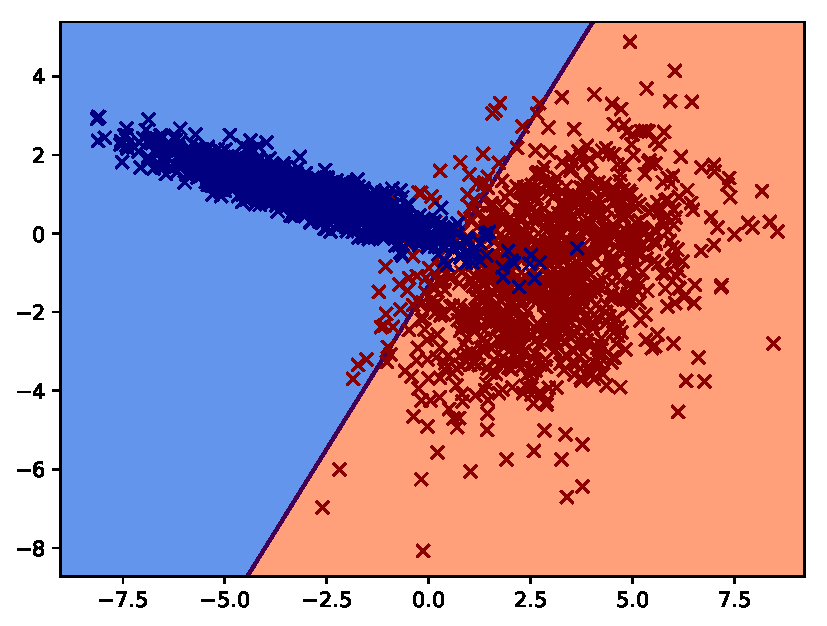
\includegraphics[width=\textwidth]{LogReg_classificationB_test.pdf}
    \caption{Test observations B ($1500$ points)}\label{fig:LogReg-B-test}
  \end{subfigure}
  \vskip\baselineskip
  \begin{subfigure}[t]{0.40\textwidth}
    \centering
    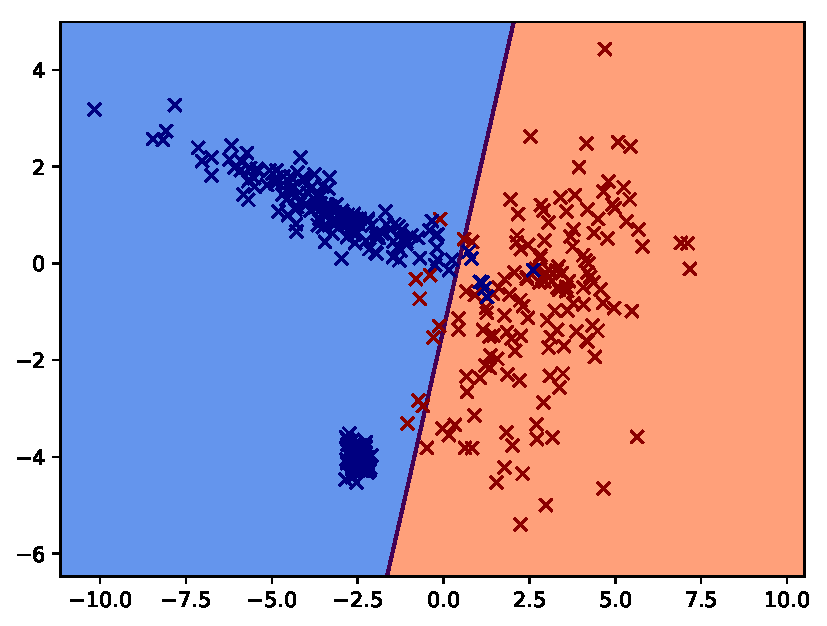
\includegraphics[width=\textwidth]{LogReg_classificationC_train.pdf}
    \caption{Training observations C ($150$ points)}\label{fig:LogReg-C-train}
  \end{subfigure}
  \quad
  \begin{subfigure}[t]{0.40\textwidth}
    \centering
    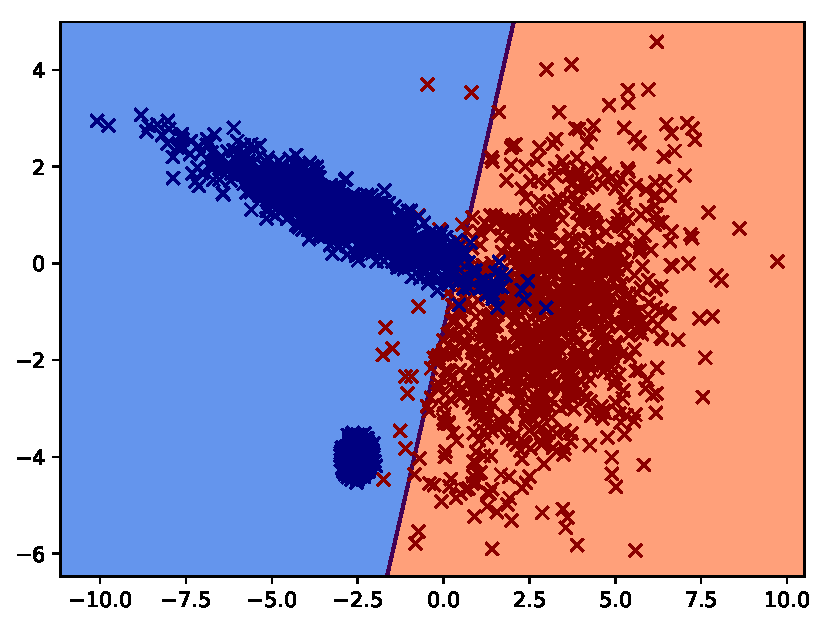
\includegraphics[width=\textwidth]{LogReg_classificationC_test.pdf}
    \caption{Test observations C ($1500$ points)}\label{fig:LogReg-C-test}
  \end{subfigure}
  \caption{Sample data and decision boundary representation for the \name{logistic regression} classifier on the three files}\label{fig:LogReg}
\end{figure}

%% End exercice

\clearpage

\subsection{Linear Regression}

\begin{question}
  I've implemented the linear regression using the normal equation
  as suggested.

  \begin{equation*}
    \hat{w} = (X^T X)^{-1} X^T y
  \end{equation*}

  \begin{equation*}
    \hat{\sigma}^2 = \dfrac{1}{N} \sum_{i = 1}^N {\left(y^{(i)} - w^T x^{(i)}\right)}
  \end{equation*}


  The values of $\hat{w}$ and $\hat{\sigma}^2$ are given for the 3 training files :

\begin{table}[h!]
    \centering
    \begin{tabular}{| l | c | c |}
      \hline
      sample file & $\hat{w}$ & $\hat{\sigma}^2$\\
      \hline
      \file{classificationA} & $(-0.26,\hspace{0.5em}-0.37,\hspace{0.5em}0.49)$ & 0.050 \\
      \file{classificationB} & $(-0.10,\hspace{0.5em}0.05,\hspace{0.5em}0.50)$  & 0.054 \\
      \file{classificationC} & $(-0.13,\hspace{0.5em}-0.02,\hspace{0.5em}0.51)$ & 0.062 \\
      \hline
    \end{tabular}
    \captionof{table}{Parameters learnt for the linear regression method for the different training sample} \label{tab:ParamLinReg}
  \end{table}



  %% \begin{minipage}{\linewidth}
  %%   \begin{lstlisting}[language=Python]
  %%     class LinearRegression(ClassificationModel):

  %%     def train(self, X, Y):
  %%     N = np.shape(X)[0]
  %%     X = np.c_[X, np.ones(N)]
  %%     K = np.linalg.inv(X.T.dot(X))
  %%     self.W = K.dot(X.T).dot(Y)

  %%     def probability(self, X):
  %%     X = np.hstack((X, 1))
  %%     return self.W.dot(X)
  %%   \end{lstlisting}
  %% \end{minipage}

\end{question}

\begin{question}
  The representation of the data and the decision boundary are represented on \Figure{fig:LinReg}

  \begin{figure}[!ht]
    \centering
    \begin{subfigure}[t]{0.40\textwidth}
      \centering
      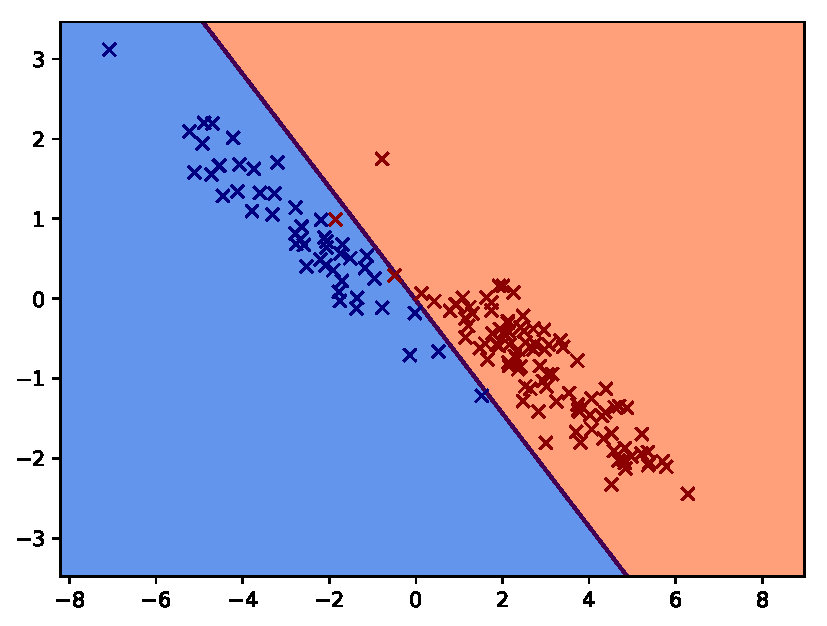
\includegraphics[width=\textwidth]{LinReg_classificationA_train.pdf}
      \caption{Training observations A ($150$ points)}\label{fig:LinReg-A-train}
    \end{subfigure}
    \quad
    \begin{subfigure}[t]{0.40\textwidth}
      \centering
      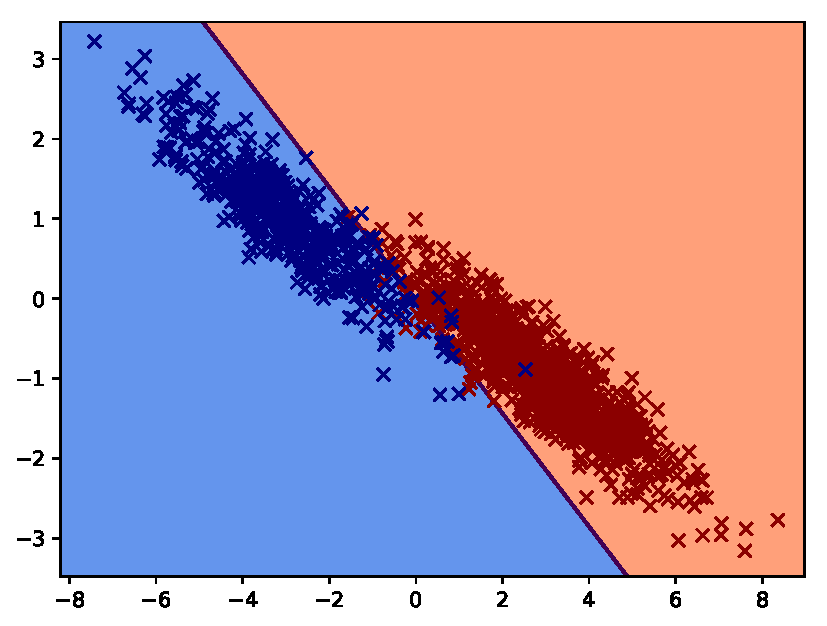
\includegraphics[width=\textwidth]{LinReg_classificationA_test.pdf}
      \caption{Test observations A ($1500$ points)}\label{fig:LinReg-A-test}
    \end{subfigure}
    \vskip\baselineskip
    \begin{subfigure}[t]{0.40\textwidth}
      \centering
      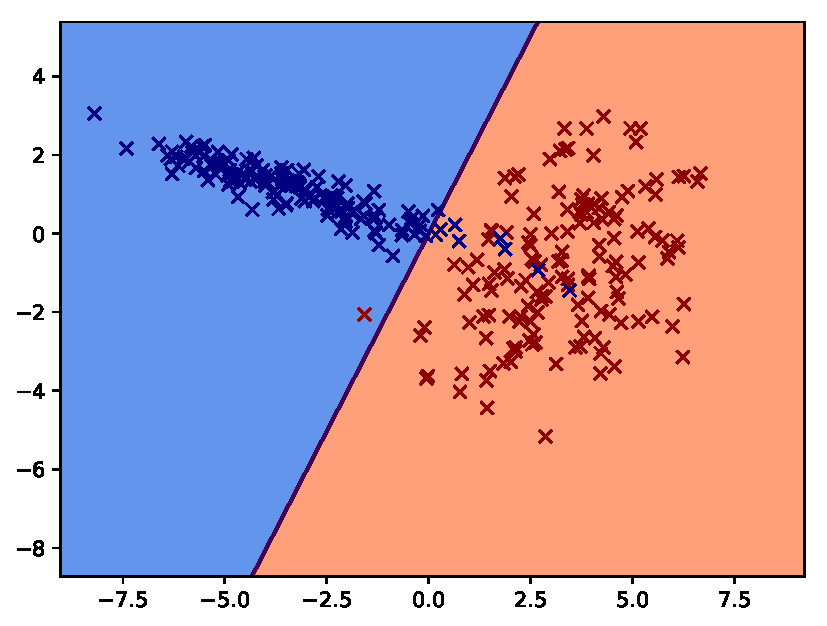
\includegraphics[width=\textwidth]{LinReg_classificationB_train.pdf}
      \caption{Training observations B ($150$ points)}\label{fig:LinReg-B-train}
    \end{subfigure}
    \quad
    \begin{subfigure}[t]{0.40\textwidth}
      \centering
      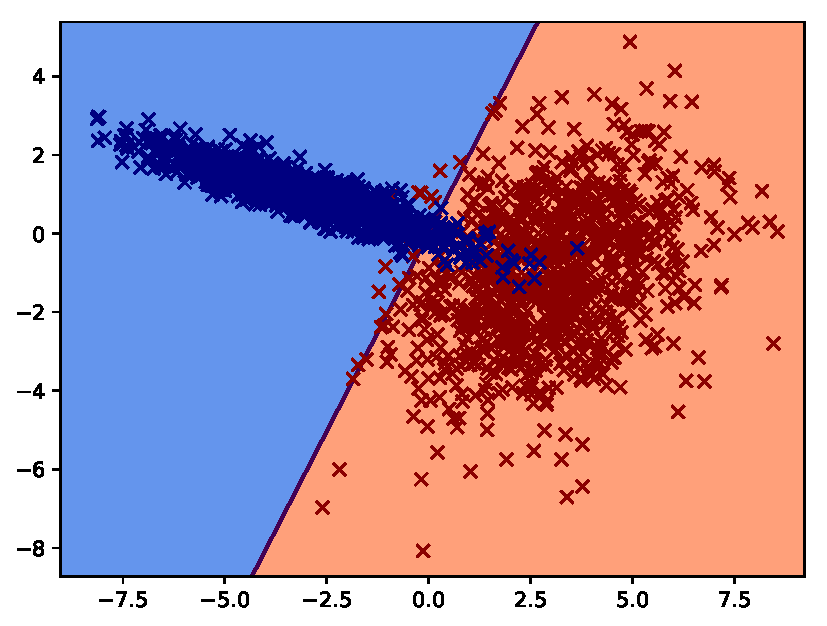
\includegraphics[width=\textwidth]{LinReg_classificationB_test.pdf}
      \caption{Test observations B ($1500$ points)}\label{fig:LinReg-B-test}
    \end{subfigure}
    \vskip\baselineskip
    \begin{subfigure}[t]{0.40\textwidth}
      \centering
      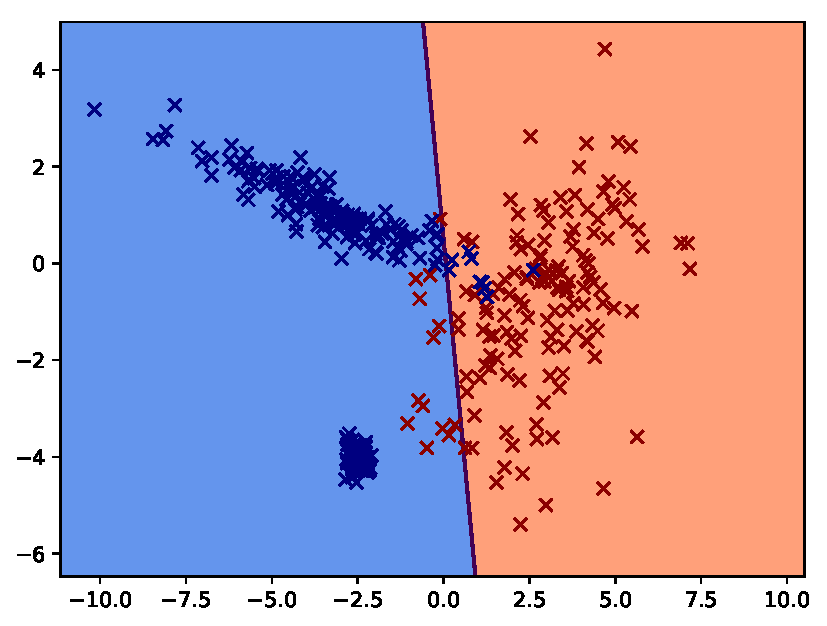
\includegraphics[width=\textwidth]{LinReg_classificationC_train.pdf}
      \caption{Training observations C ($150$ points)}\label{fig:LinReg-C-train}
    \end{subfigure}
    \quad
    \begin{subfigure}[t]{0.40\textwidth}
      \centering
      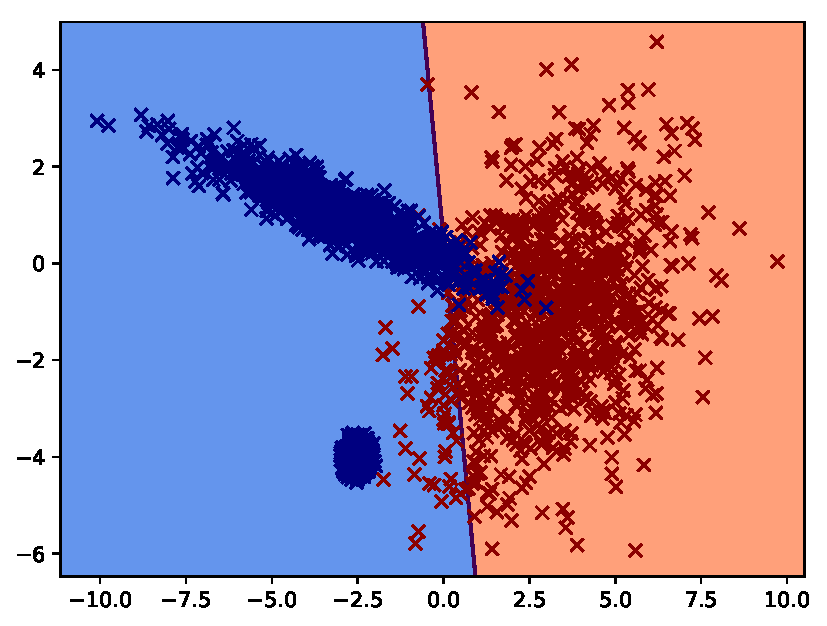
\includegraphics[width=\textwidth]{LinReg_classificationC_test.pdf}
      \caption{Test observations C ($1500$ points)}\label{fig:LinReg-C-test}
    \end{subfigure}
    \caption{Sample data and decision boundary representation for the \name{linear regression} classifier on the three files}\label{fig:LinReg}
  \end{figure}


\end{question}

%% End exercice

\subsection{Comparison of the results}

\begin{question}
  I'll first present the results I've obtained on the train and
  test data.  These results can be obtain by running the python
  script \file{classify.py} (it outputs train error and test error
  as well as the parameters for the different methods).

  Here are the results of the different methods on the 3 sample files
  presented in an array. Each cell consists of two values $E_{train}$ and
  $E_{test}$ which are respectively the misclassification error on the training
  sample and on the test sample for this file.

\begin{table}[h!]
    \centering
    \begin{tabular}{| c | c | c | c |}
      \hline
      Method & \file{classificationA} & \file{classificationB} & \file{classificationC}\\
      \hline
      LDA                 & \colgood{1.33\% / 2.00\%} & 3.00 / 4.15\%           & 5.50\% / 4.23\% \\
      Logistic Regression & 0.00\% / 3.47\%           & 2.00 / 4.30\%           & \colgood{4.00\% / 2.27\%} \\
      Linear Regression   & 1.33\% / 2.07\%           & 3.00 / 4.15\%           & 5.50\% / 4.23\% \\
      QDA                 & 0.67\% / 2.00\%           & \colgood{1.33\% / 2.00\%} & 5.25\% / 3.83\% \\
      \hline
    \end{tabular}
    \captionof{table}{Comparison of the misclassification errors (training / test) for the different methods and files} \label{tab:ErrorAll}
  \end{table}

\end{question}

\begin{question}
  For each file, the best classification method for the test
  sample is represented in green in the array.

  \ipart{SampleA}

  For the sample \name{A}, the 3 methods perform well, by looking
  at the data, we can guess that it has been generated from a
  weighted sum of 2 normal distribution with the same covariant
  matrix (and of course different means), so this is not
  surprising that the \name{LDA} performs well (the model fits the
  data perfectly). Moreover the training data is separable (we
  can see that by the logistic regression having a training
  misclassification error of $0.00$), which explains why the
  training error are very low. The test data has very little
  overlapping, which explains why all the methods performs
  well. The logistic regression induces a small overfitting on
  this sample, it matches perfectly the training samples, but has
  the worst test error.

  \ipart{SampleB}

  For the sample \name{B}, we can guess that it has also been
  generated from a weighted sum of 2 normal distribution, but this
  time with different covariant matrix. That explains why the
  \name{QDA} is outperforming the 2 other methods.

  There's an overlapping zone between the 2 gaussian kernels, which
  explains why the performance is overall worst that the SampleA, the
  3 other methods that try to fit a line (e.g. LDA, Linear Regression
  and Logistic Regression), have very similar results on the test
  sample.

  \ipart{SampleC}

  The sample C is very similar to the sample B, the only change is
  that there's an additional dense gaussian kernel whose points are
  labeled $y^{(i)} = 1$. We can notice that all 3 methods
  perform well (less than $5\%$ misclassification error on the test
  data), though none of the model fits the data perfectly.

  The logistic regression performs better on this dataset. This is a
  really interesting example, since the small dense gaussian kernel
  added from SampleB to SampleC would be in fact correctly classified
  by all the models trained with B (e.g trained without this extra data)
  What we are testing is in fact the stability of the method, and we
  expect a small change in the boundary line in order for the method to
  be stable.

  I have computed the angle between the boundary line and the x-axis
  for linear regression and logistic regression, for both SampleB and
  SampleC, the results are presented in the \Table{tab:LineAngle}.
  The first thing we can notice is that the angles for the two methods
  are similar for the file SampleB. We also see that the angle change
  between SampleB and SampleC is only $0.23$ rad for the logistic
  regression versus $0.59$ rad for the linear regression. This means
  that the logistic regression is much more stable than the linear
  regression.

\begin{table}[h!]
    \centering
    \begin{tabular}{| c | c | c | c |}
      \hline
      Method & \file{classificationB} & \file{classificationC} & difference \\
      \hline
      Linear Regression & 1.11 rad / 63 deg  & 1.70 rad / 98 deg & 0.59 rad / 34 deg \\
      Logistic Regression & 1.03 rad / 59 deg & 1.26 rad / 72 deg & 0.23 rad / 13 deg \\
      \hline
    \end{tabular}
    \captionof{table}{Comparison of the angles between the boundary line and the x-axis for the files \file{classificationB} and \file{classificationC} } \label{tab:LineAngle}
  \end{table}

%% >>> math.atan2(-0.10424575, -0.05179118)
%% 1.1096974412187182
%% >>> math.atan2(-0.12769333, 0.01700142)
%% 1.7031604375912033
%% >>> math.atan2(1.70518586, 1.02378538)
%% 1.0300862999245632
%% >>> math.atan2(2.2032324, 0.70926562)
%% 1.2593522694822836
%% >>> np.abs(1.1096974412187182 - 1.7031604375912033)
%% 0.59346299637248512
%% >>> np.abs(1.0300862999245632 - 1.2593522694822836)
%% 0.22926596955772038

  %% Intuitively, adding this region of points shifts $\mu_0$ for the LDA,
  %% which rotates the boundary line.



\end{question}

%% End exercice

\clearpage

\subsection{QDA model}

\begin{question}
  For the QDA model, we can generalize the expression of the
  likelihood found for the QDA.

  \begin{equation*}
    p(x^{(i)} | y^{(i)}) = \dfrac{1}{\sqrt{(2 \pi)^d \det{\Sigma_{y^{(i)}}}}}\exp{\left( -\dfrac{1}{2} (x^{(i)} - \mu_{y^{(i)}})^T \Sigma_{y^{(i)}}^{-1} (x^{(i)} - \mu_{y^{(i)}}) \right)}
  \end{equation*}

  We obtain this expression for the log likelihood

  %% \begin{equation*}
  %%   \begin{split}
  %%     \ln{\mathcal{L}(\theta)} & = - \dfrac{d N}{2}\ln{(2\pi)} \\
  %%     & + \sum_{i = 1}^N \left( y^{(i)} \ln{(\pi)} + (1 - y^{(i)})\ln{(1 - \pi)} \right) \\
  %%     & + \sum_{i = 1}^N \left( - \dfrac{1}{2} y^{(i)} \det{\Sigma_1} - \dfrac{1}{2} (1 - y^{(i)}) \det{\Sigma_0} \right)\\
  %%     & + \sum_{i = 1}^N \left( y^{(i)} (x^{(i)} - \mu_1)^T \Sigma_1^{-1} (x^{(i)} - \mu_1) + (1 - y^{(i)}) (x^{(i)} - \mu_0)^T \Sigma_0^{-1} (x^{(i)} - \mu_0) \right)
  %%   \end{split}
  %% \end{equation*}

  \begin{equation*}
    \begin{split}
      \ln{\mathcal{L}(\theta)} & = - \dfrac{d N}{2}\ln{(2\pi)} \\
      & + \sum_{i = 1}^N \left( y^{(i)} \ln{(\pi)} + (1 - y^{(i)})\ln{(1 - \pi)} \right) \\
      & - \dfrac{1}{2} \sum_{i = 1}^N y^{(i)} \left( \ln{\det{\Sigma_1}} + (x^{(i)} - \mu_1)^T \Sigma_1^{-1} (x^{(i)} - \mu_1) \right)\\
      & - \dfrac{1}{2} \sum_{i = 1}^N (1 - y^{(i)}) \left( \ln{\det{\Sigma_0}} + (x^{(i)} - \mu_0)^T \Sigma_0^{-1} (x^{(i)} - \mu_0) \right)\\
    \end{split}
  \end{equation*}

  We see that the maximum likelihood estimator for $\pi$, $\mu_0$
  and $\mu_1$ are identical for the QDA and the LDA.


  Moreover, using the same notation that we used for the LDA,
  we can obtain the maximum likelihood estimators for
  $\Sigma_0$ and $\Sigma_1$ as follows

  \begin{equation*}
    \hat{\Sigma}_j = \dfrac{1}{N_j} \sum_{i = 0}^N \delta_{j, y^{(i)}} (x^{(i)} - \mu_j)(x^{(i)} - \mu_j)^T
  \end{equation*}

  The values obtained from my implementation of the QDA are
  represented in the following table

  %% 0.333333333333 & ( 2.89970947, -0.893874 ) & ( -2.69232004, 0.866042  ) &
  %% \begin{array}{ll}
  %%    2.33399251 & -1.05806527 \\
  %%    -1.05806527 &  0.58160003 \\
  %% \end{array} &
  %% \begin{array}{ll}
  %%    2.759614 &   -1.32739949 \\
  %%    -1.32739949 &  0.70377131 \\
  %% \end{array} \\

  %% 0.5 & ( 3.34068896, -0.83546333 ) & ( -3.21670734, 1.08306733) &
  %% \begin{array}{ll}
  %%    2.55589791 &  1.07135355 \\
  %%    1.07135355 &  2.97994521 \\
  %% \end{array} &
  %% \begin{array}{ll}
  %%    4.18148733 & -1.34349762 \\
  %%    -1.34349762 &  0.51953415 \\
  %% \end{array} \\

  %% 0.625 & ( 2.79304824, -0.83838667 ) & ( -2.94232885,-0.9578284 ) &
  %% \begin{array}{ll}
  %%   2.91859658 &  1.25417671 \\
  %%   1.25417671 &  2.9443837  \\
  %% \end{array} &
  %% \begin{array}{ll}
  %%   2.8806667 &  -1.76904679 \\
  %%   -1.76904679 &  6.59074926 \\
  %% \end{array} \\




  \begin{table}[h!]
    \centering
  \begin{tabular}{| l | l | l | l | c | c |}
    \hline
    sample file & $\pi$ & $\mu_0$ & $\mu_1$ & $\Sigma_0$ & $\Sigma_1$ \\
    \hline
    \file{classificationA} &
    0.33 & ( 2.90, -0.89 ) & ( -2.69, 0.87  ) &
    \( \left( \begin{array}{cc}
      2.33 & -1.06 \\
      -1.06 &  0.58
    \end{array} \right) \) &
    \( \left( \begin{array}{cc}
      2.76 & -1.33 \\
      -1.33 &  0.70 \\
    \end{array} \right) \) \\

    \file{classificationB} &
    0.5 & ( 3.34, -0.84 ) & ( -3.22, 1.08) &
    \( \left( \begin{array}{cc}
      2.56 &  1.07 \\
      1.07 &  2.98 \\
    \end{array} \right)  \) &
    \( \left( \begin{array}{cc}
      4.18 & -1.34 \\
      -1.34 &  0.52 \\
    \end{array} \right)  \) \\

    \file{classificationC} &
    0.625 & ( 2.79, -0.84 ) & ( -2.94,-0.96 ) &
    \( \left( \begin{array}{cc}
      2.92 &  1.25 \\
      1.25 &  2.94  \\
    \end{array} \right)  \) &
    \( \left( \begin{array}{cc}
      2.88 &  -1.77 \\
      -1.77 &  6.59 \\
    \end{array} \right)  \) \\
    \hline
  \end{tabular}
  \captionof{table}{Parameters learnt for the QDA method for the different training sample} \label{tab:ParamQDA}
\end{table}


\end{question}
\begin{question}
  The sample data and decision boundary of this classifier are represented on \Figure{fig:QDA}

  \begin{figure}[!ht]
    \centering
    \begin{subfigure}[t]{0.40\textwidth}
      \centering
      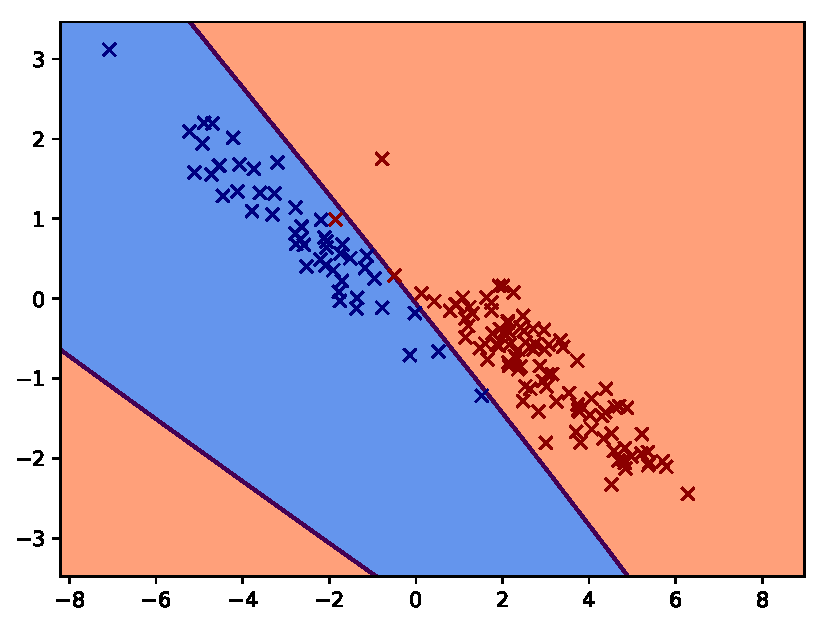
\includegraphics[width=\textwidth]{QDA_classificationA_train.pdf}
      \caption{Training observations A ($150$ points)}\label{fig:QDA-A-train}
    \end{subfigure}
    \quad
    \begin{subfigure}[t]{0.40\textwidth}
      \centering
      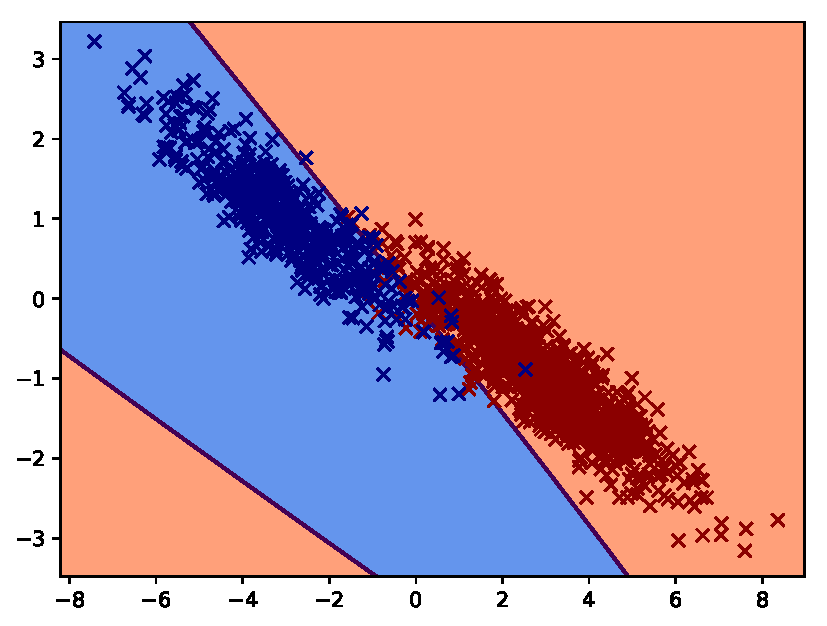
\includegraphics[width=\textwidth]{QDA_classificationA_test.pdf}
      \caption{Test observations A ($1500$ points)}\label{fig:QDA-A-test}
    \end{subfigure}
    \vskip\baselineskip
    \begin{subfigure}[t]{0.40\textwidth}
      \centering
      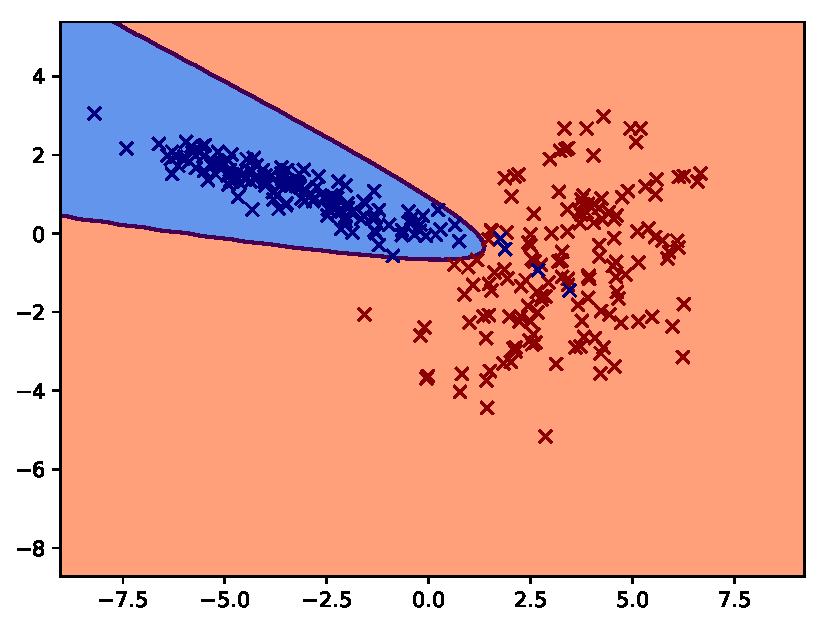
\includegraphics[width=\textwidth]{QDA_classificationB_train.pdf}
      \caption{Training observations B ($150$ points)}\label{fig:QDA-B-train}
    \end{subfigure}
    \quad
    \begin{subfigure}[t]{0.40\textwidth}
      \centering
      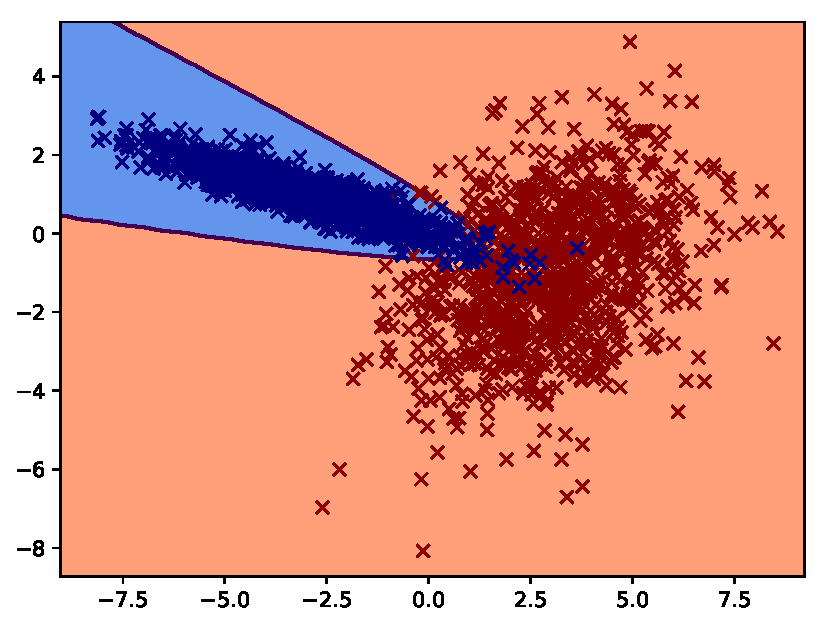
\includegraphics[width=\textwidth]{QDA_classificationB_test.pdf}
      \caption{Test observations B ($1500$ points)}\label{fig:QDA-B-test}
    \end{subfigure}
    \vskip\baselineskip
    \begin{subfigure}[t]{0.40\textwidth}
      \centering
      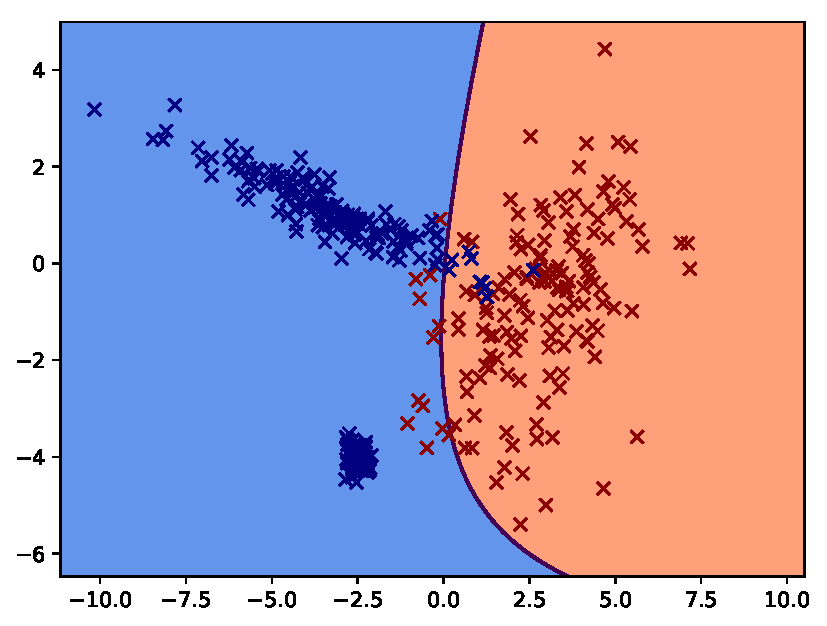
\includegraphics[width=\textwidth]{QDA_classificationC_train.pdf}
      \caption{Training observations C ($150$ points)}\label{fig:QDA-C-train}
    \end{subfigure}
    \quad
    \begin{subfigure}[t]{0.40\textwidth}
      \centering
      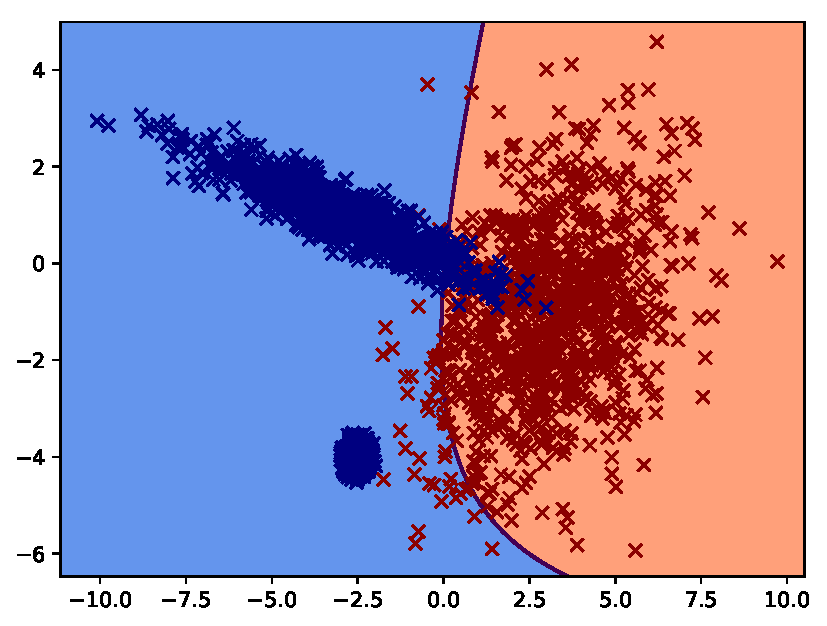
\includegraphics[width=\textwidth]{QDA_classificationC_test.pdf}
      \caption{Test observations C ($1500$ points)}\label{fig:QDA-C-test}
    \end{subfigure}
    \caption{Sample data and decision boundary representation for the \name{QDA} classifier on the three files}\label{fig:QDA}
  \end{figure}

\end{question}

\begin{question}
  \Table{tab:ErrorQDA} presents the misclassification error for both training and test sample (it's also present in \Table{tab:ErrorAll}, which regroups the misclassification error for all methods)

  \begin{table}[h!]
    \centering
    \begin{tabular}{| c | c | c | c |}
      \hline
      Method & \file{classificationA} & \file{classificationB} & \file{classificationC}\\
      \hline
      Training error & 0.67\% & 1.33\% & 5.25\% \\
      Test error & 2.00\% & 2.00\% & 3.83\% \\
      \hline
    \end{tabular}
    \captionof{table}{Comparison of the training and test misclassification error for the QDA on the different training sample} \label{tab:ErrorQDA}
  \end{table}

\end{question}

\begin{question}
  The QDA method provides the overall best results in particular for
  samples B and C. It's no suprise that it performs better than the
  LDA, since the LDA is a particular case of the QDA when $\Sigma_0 =
  \Sigma_1$, we can see that on the \Table{tab:ParamQDA}, the 2 matrix
  found are very close $\norm{\Sigma_0 - \Sigma_1}^2 \approx 0.341$,
  and we observe in the \Figure{fig:QDA-A-train} and
  \Figure{fig:QDA-A-test} that the decision boundary is approximately
  a line.

\end{question}


\section{Implementation details}

I've implemented the 4 classifiers (LDA, QDA, Linear Regression and
Logistic Regression) in Python. The script is located in the file
\file{src/classify.py}, it trains all classifiers on the files
\file{data/classificationA.train}, \file{data/classificationB.train},
\file{data/classificationC.train} compute and print the parameters, and
test the trained classifier on the files \file{data/classificationA.test},
\file{data/classificationB.test}, \file{data/classificationC.test} it then
computes and outputs the train and the test misclassification error It
also save graphs under \file{imgs/} showing for each classifier and
each file, the data sample and the decision boundary.

Each classifier corresponds to a class that inherit the class
\name{ClassificationModel}. This class is responsible for classifying
and plot the contour of data based on the subclasses overriding the
function \name{probability}. Each classifier class has 3 methods :
\name{train} which is used for training the classifier,
\name{probability} which estimates the probability that a given point
$X$ belongs to class $1$, and \name{print\_params} which prints the
parameters of the model.

There's also a script that generates data sample from two gaussian
kernels \file{generate.py} that I used to check and to experiment
the classification methods (it's not very user friendly but I let
it in the archive nonetheless).


\section{Conclusion}

This homework was interesting and visual, I really enjoyed doing
it. This was also the opportunity for me to learn Python, I've tried
to make a code as clear as possible though there's not much comments
in the code... I should also have implemented a stopping criterion for
the Newton-Raphson method on Logistic regression, (I chose a fixed
number of iterations) a decent criterion would be to stop when the
gradient is sufficiently small.

\end{document}
